% scritto da Tommaso Azzalin
\section{Strategia di testing}
Il gruppo \Gruppo{} per assicurarsi che il prodotto da realizzare sia corretto intende effettuare un piano di testing delle componenti e del sistema software nel suo complesso.
L'obiettivo è seguire il modello a V per correlare ogni attività di testing (parte destra della V) con la corrispondente attività della parte sinistra della V.

\begin{figure}[h]
    \centering
    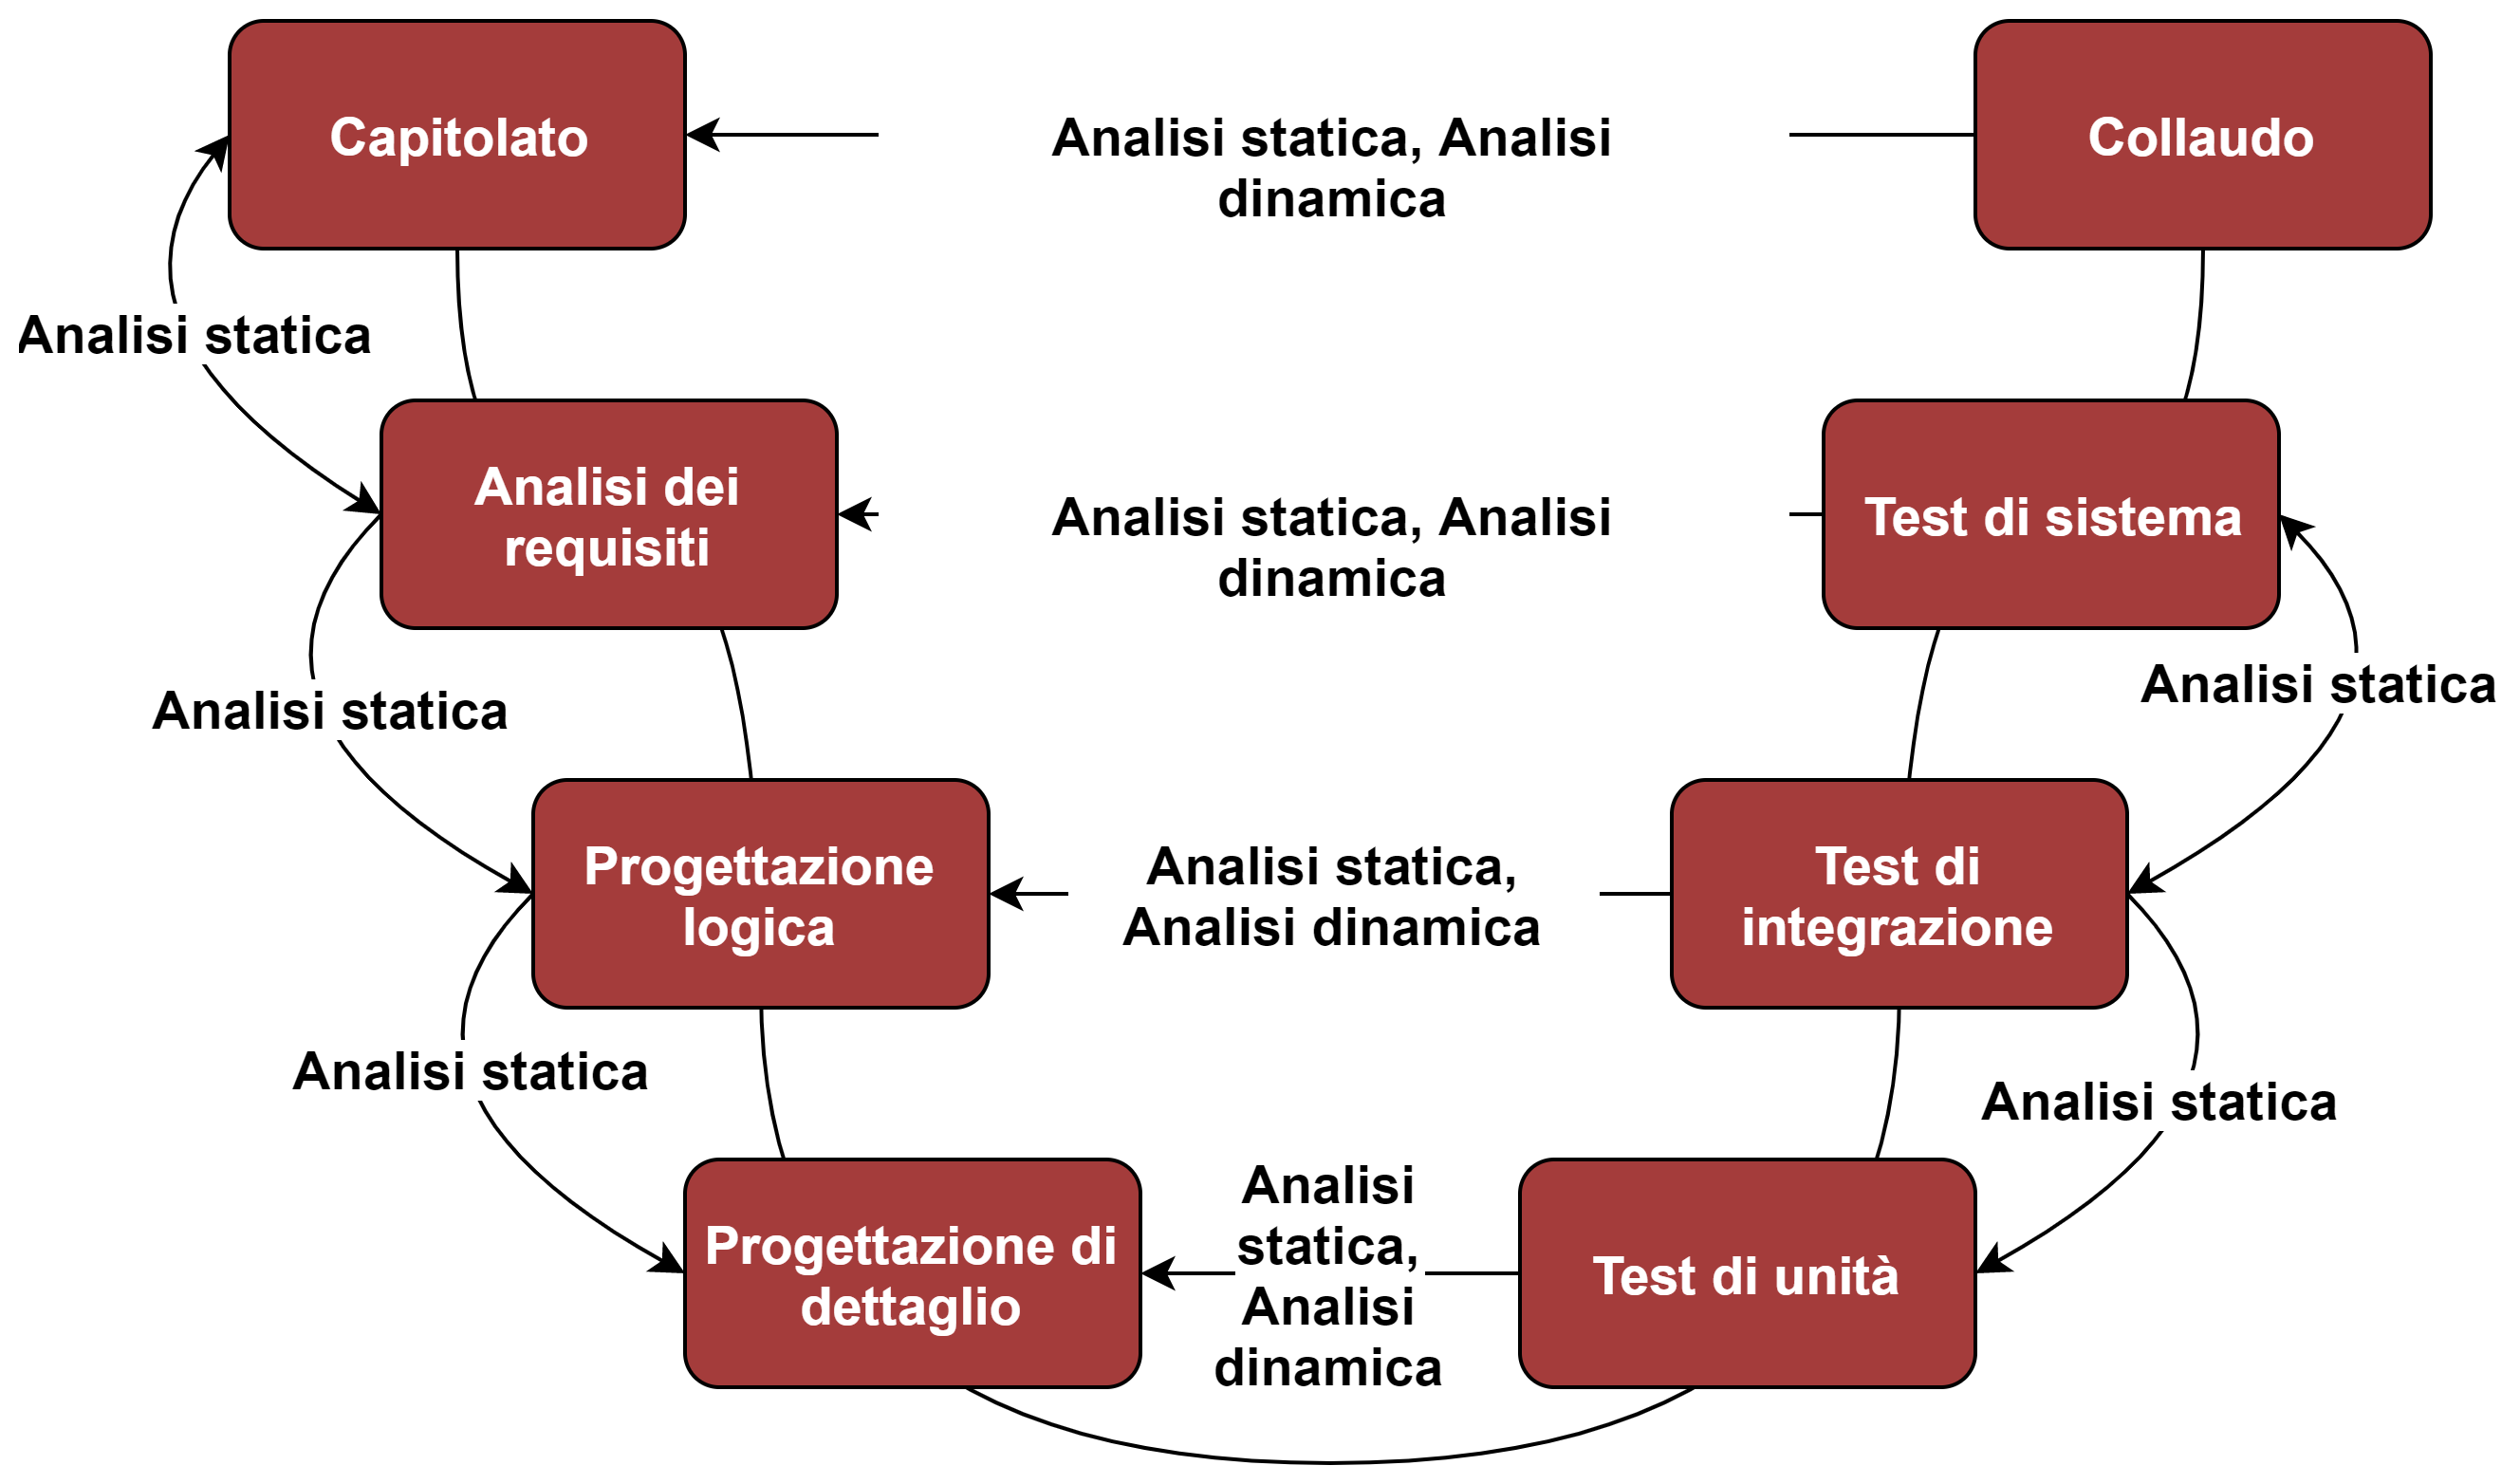
\includegraphics[scale=0.85]{sezioni/Immagini/Modello_a_V.png}
    \caption{Modello a V}
\end{figure}

\subsection{Tipologie di test}
I test specificati dal modello a V e che devono essere realizzati dal gruppo sono:
\begin{itemize}
    \item \textbf{Test di unità:} verificano il corretto comportamento di una singola unità del programma. L'unità è una funzionalità atomica verificabile in modo isolato, in modo da assicurare che il risultato dei test su essa non siano influenzati dal comportamento di altre unità. 
    \item \textbf{Test di integrazione:} verificano il corretto comportamento di più unità che devono cooperare per svolgere a pieno i loro compiti.
    \item \textbf{Test di sistema:} verificano il comportamento dell'intero sistema. I requisiti funzionali, di vincolo, di qualità e di prestazione concordati alla stipulazione del contratto con il committente devono essere soddisfatti per intero.
    \item \textbf{Test di accettazione:} vengono eseguiti assieme al committente e un loro superamento permettono di procedere con il rilascio del prodotto software.
\end{itemize}

\subsubsection{Test di unità}
Allo stato attuale del progetto non è possibile definire quali test di unità dovranno essere realizzati, in quanto devono essere realizzati in contemporanea alla progettazione di dettaglio.
Questa sezione del documento verrà redatta non appena inizierà l'attività di progettazione di dettaglio.

\subsubsection{Test di integrazione}
Allo stato attuale del progetto non è possibile definire quali test di integrazione dovranno essere realizzati, in quanto devono essere realizzati in contemporanea alla progettazione di dettaglio.
Questa sezione del documento verrà redatta non appena inizierà l'attività di progettazione di dettaglio.

\subsubsection{Test di sistema}
I test di sistema devono assicurare la completa copertura dei requisiti espressi nel documento \textit{Analisi dei Requisiti}.
Ogni test di sistema è identificato da un codice, così formato:
\begin{center}
    TS-[Importanza][Tipologia][Codice]
\end{center}
con:
\begin{itemize}
    \item \textbf{[Importanza]:}
    \begin{itemize}
        \item \textbf{1}: il test verifica il funzionamento di un requisito obbligatorio;
        \item \textbf{2}: il test verifica il funzionamento di un requisito desiderabile;
        \item \textbf{3}: il test verifica il funzionamento di un requisito opzionale;
    \end{itemize}
    \item \textbf{{Tipologia}:}
    \begin{itemize}
        \item \textbf{F}: il requisito di riferimento è funzionale;
        \item \textbf{Q}: il requisito di riferimento è qualitativo;
        \item \textbf{P}: il requisito di riferimento è prestazionale;
        \item \textbf{V}: il requisito di riferimento è un vincolo;
    \end{itemize}
    \item \textbf{[Codice]:}
    \begin{itemize}
        \item \textbf{A$u.v$} il requisito di riferimento riguarda l'applicazione, in cui $u$ indica il numero del caso d'uso (lato app) kite-level di provenienza, $u$ il numero progressivo univoco;
        \item \textbf{S$w.x$} il requisito di riferimento riguarda l'applicazione, in cui $w$ indica il numero del caso d'uso (lato serve) kite-level di provenienza, $x$ il numero progressivo univoco;
        \item \textbf{C$y$} il requisito proviene dal capitolato, dove $y$ sarà il numero progressivo univoco;
        \item \textbf{V*} il requisito proviene da un verbale, dove * inizierà con I se proviene da un verbale interno oppure E se proviene da un verbale esterno. Poi vi sarà il numero che indica il verbale da cui proviene il requisito; il numero si calcola a partire da 1, che sarà associato al primo verbale redatto (in ordine temporale). I numeri per i verbali interni sono contati separatamente da quelli dei verbali esterni. Infine vi sarà un punto seguito dal numero progressivo
        \item \textbf{I$z$} il requisito proviene da una decisione presa internamente al gruppo, dove $z$ sarà un numero progressivo.
    \end{itemize}
\end{itemize}

Segue l'elenco dei test con la relativa descrizione.

{
\rowcolors{2}{grigetto}{white}
\renewcommand{\arraystretch}{1.5}
\centering
\begin{longtable}{ c  C{2.5cm}  C{10cm} C{1cm}}
\caption{Elenco dei test di sistema}\\
\rowcolor{darkblue}
\textcolor{white}{\textbf{Codice}} & \textcolor{white}{\textbf{Titolo}} & \textcolor{white}{\textbf{Descrizione}} & \textcolor{white}{\textbf{Stato}}\\
\endfirsthead
\rowcolor{darkblue}
\textcolor{white}{\textbf{Codice}} & \textcolor{white}{\textbf{Titolo}} & \textcolor{white}{\textbf{Descrizione}} & \textcolor{white}{\textbf{Stato}}\\
\endhead

%da R1FI1 a R1FA8.4 (con parti splittate) % Christian
TSA1 & Accesso all'applicazione di un utente non autenticato con credenziali Stalker &
Verificare che l'utente non autenticato:
\begin{enumerate}
    \item Possa inserire l'indirizzo e-mail;
    \item Possa inserire la password;
    \item Riceva un messaggio di errore se l'\glo{autenticazione} viene negata per inserimento di credenziali errate.
\end{enumerate}
Se l'utente non autenticato si è dimenticato la sua password:
\begin{enumerate}[resume]
    \item Verifica che l'utente non autenticato possa effettuare il reset della password qualora se la fosse dimenticata.
\end{enumerate} & ?? \\

%da R1FI1 a R1FA8.4 (con parti splittate) % Christian
TSA2 & Registrazione nell'applicazione di un utente non autenticato con credenziali Stalker &
Verificare che l'utente non autenticato:
\begin{enumerate}
    \item Possa inserire l'indirizzo e-mail;
    \item Riceva un messaggio di errore se tentasse di registrarsi con un'e-mail già usata nel sistema;
    \item Possa inserire una password;
    \item Possa inserire nuovamente la password come conferma;
    \item Riceva un messaggio di errore qualora abbia inserito una password non ritenuta sicura. Il processo di \glo{autenticazione} deve fallire;
    \item Riceva un messaggio di errore qualora abbia inserito una conferma password diversa dalla password. Il processo di \glo{autenticazione} deve fallire;
    \item Possa accettare le condizioni generali d'uso;
    \item La registrazione si interrompa e che l'applicazione si chiuda nel caso che l'utente non autenticato non abbia accettato le condizioni generali d'uso.
\end{enumerate} & ?? \\

% R1FA2.1
TSA3  & \glo{Logout} dell'utente anonimo & \begin{enumerate}
    \item Verifica che l'utente anonimo possa effettuare il \glo{logout} dall'applicazione.
\end{enumerate} & ?? \\

% da R1FA3.1, R1FA3.2, R1FA8.5, R1FA3.7, R1FA3.8, R1FA3.9 % Riccardo
TSA4 & Gestione lista delle \glo{organizzazioni} &
Verificare che l'utente anonimo:
\begin{enumerate}
    \item Possa scaricare la lista di tutte le organizzazioni;
    \item Riceva un messaggio di errore qualora lo scaricamento della lista di tutte le organizzazioni non vada a buon fine;
    \item Possa aggiornare la lista delle organizzazioni tramite \glo{refresh manuale};
    \item Possa aggiornare la lista delle organizzazioni tramite \glo{temporizzazione}.
\end{enumerate} & ?? \\

% R1FA3.10, R1FA3.11, R1FA3.12, R1FA3.13, R1FA3.14, R1FA3.15, R1FA3.16, R1FA3.17, R1FA3.18 % Riccardo
TSA5 & Visualizzazione lista delle organizzazioni & 
Verificare che l'utente anonimo:
\begin{enumerate}
% \item Possa autenticarsi con credenziali LDAP, qualora scaricasse una organizzazione che richieda l'autenticazione con credenziali LDAP;
    \item Possa visionare la lista delle organizzazioni ordinate alfabeticamente;
    \item Possa visionare la lista delle organizzazioni ordinate secondo la politica \glo{FIFO};
    \item Possa visionare la lista delle organizzazioni che permettono il tracciamento anonimo;
    \item Possa visionare la lista delle organizzazioni che permettono il \glo{tracciamento autenticato};
    \item Possa ricercare organizzazioni presenti nella lista delle organizzazioni appartenenti alle nazioni indicate dall'utente;
    \item Possa ricercare organizzazioni presenti nella lista delle organizzazioni che hanno nel nome una sotto-stringa scelta dall'utente;
    \item Possa ricercare organizzazioni presenti nella lista delle organizzazioni appartenenti alla città indicata dall'utente.
\end{enumerate} & ?? \\

% da R1FA3.3, R1FA3.4, R1FA3.5, R1FA3.6, R1FA8.6 % Riccardo
TSA6 & Gestione lista delle organizzazioni preferite dell'utente anonimo &
Verificare che l'utente anonimo:
\begin{enumerate}
    \item Possa inserire un'organizzazione, presente nella lista di tutte le organizzazioni, nella propria lista delle organizzazioni preferite;
    \item Possa rimuovere un'organizzazione dalla propria lista delle organizzazioni preferite;
    \item Venga informato nel caso in cui non sia memorizzata nessuna lista delle organizzazioni del proprio dispositivo.
\end{enumerate} & ?? \\

% da R1FA4.1 a R1FA4.3 % Tommaso
TSA7 & Selezione della modalità di \glo{tracciamento} & 
\glo{Verificare} che l'utente riconosciuto:
\begin{enumerate}
    \item Possa inserire la modalità di \glo{tracciamento anonimo};
    \item Possa inserire la modalità di \glo{tracciamento autenticato}.
\end{enumerate}
Se l'utente riconosciuto si trova presso un luogo di un'\glo{organizzazione}, \glo{verificare} che:
\begin{enumerate}[resume]
    \item Nel passaggio dalla modalità di \glo{tracciamento autenticato} a quella anonima venga inviata al sistema la richiesta di uscita dell'utente riconosciuto dal luogo e la successiva richiesta di ingresso di utente anonimo;
    \item Nel passaggio dalla modalità di \glo{tracciamento anonimo} a quella autenticata venga inviata al sistema la richiesta di uscita dell'utente anonimo dal luogo e la successiva richiesta di ingresso di utente riconosciuto.
\end{enumerate} & ?? \\

% da R2FA5.1 a R2FA5.5, da R2FA5.10 a R2FA5.12, R2FA5.16, R2FA8.5 % Tommaso
TSA8 & \glo{storico degli accessi} dell'utente anonimo presso un'\glo{organizzazione} & 
\glo{Verificare} che l'utente anonimo:
\begin{enumerate}
    \item Possa vedere il proprio storico accessi presso un'\glo{organizzazione}. Ogni accesso deve mostrare la data in cui è stato compiuto, il luogo corrispondente, il tempo totale trascorso all'interno nel luogo;
    \item come al punto 1, ma la \glo{lista degli accessi} deve risultare ordinata \glo{per data in ordine decrescente};
    \item come al punto 1, ma la \glo{lista degli accessi} deve risultare ordinata \glo{per data in ordine crescente};
    \item come al punto 1, ma della lista vengono mostrati solo gli accessi che rispettano i parametri di ricerca sul giorno cercato;
    \item Riceva un messaggio informativo in assenza di accessi effettuati presso un'\glo{organizzazione}.
\end{enumerate}
Se l'utente anonimo si trova presso un luogo dell'\glo{organizzazione}, \glo{verificare} che:
\begin{enumerate}[resume]
    \item Possa visionare il nome dello specifico luogo in cui si trova e il tempo trascorso da quando ha fatto l'ultimo ingresso;
\end{enumerate} & ?? \\

% da R2FA5.6 a R2FA5.9, da R2FA5.13 a R2FA5.15, R2FA5.17, R2FA8.6 % Tommaso
TSA9 & \glo{storico degli accessi} dell'utente anonimo presso un luogo di un'\glo{organizzazione} & 
\glo{Verificare} che:    
\begin{enumerate}
    \item L'utente anonimo possa vedere il proprio storico accessi presso il luogo di un'\glo{organizzazione}. Ogni accesso deve mostrare la data in cui è stato compiuto, il luogo corrispondente, il tempo totale trascorso all'interno nel luogo;
    \item Come al punto 1, ma la \glo{lista degli accessi} deve risultare ordinata \glo{per data in ordine decrescente};
    \item Come al punto 1, ma la \glo{lista degli accessi} deve risultare ordinata \glo{per data in ordine crescente};
    \item Come al punto 1, ma della lista vengono mostrati solo gli accessi che rispettano i parametri di ricerca sul giorno cercato;
    \item In assenza di accessi effettuati presso il luogo di un'\glo{organizzazione} selezionato l'utente anonimo visualizzi un messaggio informativo.
\end{enumerate}
Se l'utente anonimo si trova presso lo stesso luogo, \glo{verificare} che:
\begin{enumerate}[resume]
    \item L'utente anonimo possa visualizzare il tempo trascorso all'interno del luogo dall'ultimo ingresso effettuato.
\end{enumerate} & ?? \\

%da R2FA6.1 a R2FA6.9 % Christian
TSA10 & \glo{Tracciamento} dell'utente anonimo/riconosciuto nei luoghi di un'\glo{organizzazione} &
Verificare che l'utente anonimo/riconosciuto:
\begin{enumerate}
    \item Riceva la notifica della corretta registrazione se il tracciamento del suo \glo{movimento} in/da un \glo{luogo} ha avuto successo;
    \item Riceva un messaggio di errore qualora il tracciamento del \glo{movimento} non sia andato a buon fine.
\end{enumerate}
Durante la registrazione del \glo{tracciamento} del \glo{movimento} dell'utente anonimo/riconosciuto:
\begin{enumerate}[resume]
    \item Venga memorizzato il \glo{timestamp} in cui è avvenuto il \glo{movimento}.
\end{enumerate}
Se l'utente riconosciuto è in modalità di \glo{tracciamento autenticato} verificare che:
\begin{enumerate}[resume]
    \item Venga verificata la correttezza delle credenziali \glo{LDAP};
    \item Possa effettuare un ingresso in un luogo dell'\glo{organizzazione};
    \item Possa effettuare un'uscita da un luogo dell'\glo{organizzazione}.
\end{enumerate}
Se l'utente anonimo/riconosciuto è in \glo{modalità di tracciamento anonimo}:
\begin{enumerate}[resume]
    \item Possa effettuare un ingresso in un luogo dell'\glo{organizzazione};
    \item Possa effettuare un'uscita da un luogo dell'\glo{organizzazione}.
\end{enumerate} & ?? \\

%R1FA7.1 a R1FA7.3 % Riccardo
TSA11 & Autenticazione con credenziali \glo{LDAP} &
Verificare che l'utente anonimo:
\begin{enumerate}
    \item Possa autenticarsi con credenziali aziendali in un'organizzazione che richiede il tracciamento riconosciuto;
    \item Riceva un messaggio di errore qualora le credenziali \glo{LDAP} non fossero riconosciute dal server;
    \item Possa inserire il proprio nome utente durante l'autenticazione con le credenziali \glo{LDAP} aziendali;
    \item Possa inserire la propria password durante l'autenticazione con le credenziali \glo{LDAP} aziendali.
\end{enumerate} & ?? \\

% da R1FI2 a R1FS1.3 % Tommaso
TSS1 & Accesso al server di un amministratore non autenticato & 
\glo{Verificare} che l'amministratore non \glo{autenticato}:
\begin{enumerate}
    \item Possa inserire l'e-mail correttamente;
    \item Possa inserire correttamente la password;
    \item Riceva un messaggio d'errore se l'\glo{autenticazione} viene negata per inserimento di credenziali errate.
\end{enumerate}
Se l'amministratore non \glo{autenticato} si è dimenticato della password, \glo{verificare} che:
\begin{enumerate}[resume]
    \item L'amministratore non \glo{autenticato} possa effettuare il reset della password qualora se la fosse dimenticata.
\end{enumerate} & ?? \\

%R1FS2.1 % Tommaso
TSS2 & \glo{Logout} dell'amministratore \glo{autenticato} & \begin{enumerate}
    \item \glo{Verificare} che l'amministratore \glo{autenticato} possa effettuare il \glo{logout} dal server.
\end{enumerate} & ?? \\

%da R1FC3 a R1FI8 % Christian
TSS3 & Disponibilità \glo{organizzazioni} visualizzabili dall'amministratore &
Verificare che l'amministratore possa:
\begin{enumerate}
    \item Vedere il suo nome dell'organizzazione;
    \item Vedere l'immagine dell'organizzazione;
    \item Possa selezionare l'organizzazione;
    \item Possa selezionare l'organizzazione e vederne il nome;
    \item Possa selezionare l'organizzazione e vederne l'immagine;
    \item Possa selezionare l'organizzazione e vederne la descrizione;
    \item Possa selezionare l'organizzazione e vederne l'indirizzo.
\end{enumerate} & ?? \\

% R1FS4.1 a R1FS4.11 % Riccardo
TSS4 & Modifica dei dati dell'organizzazione &
Verificare che l'amministratore gestore:
\begin{enumerate}
    \item Possa modificare il nome dell'organizzazione;
    \item Possa modificare l'immagine della organizzazione;
    \item Possa modificare la descrizione dell’organizzazione;
    \item Possa modificare l'indirizzo dell’organizzazione;
    \item Possa modificare l'indirizzo IP dell'organizzazione;
    \item Riceva un messaggio di errore qualora il nome dell'organizzazione inserito non rispetti i vincoli imposti;
    \item Riceva un messaggio di errore qualora il nome dell'organizzazione inserito sia già presente nel sistema e associato ad un'altra organizzazione;
    \item Riceva un messaggio di errore qualora l'immagine dell'organizzazione inserita non rispetti i vincoli imposti;
    \item Riceva un messaggio di errore qualora la descrizione dell'organizzazione inserita non rispetti i vincoli imposti;
    \item Riceva un messaggio di errore qualora l'indirizzo dell'organizzazione inserito non rispetti i vincoli imposti;
    \item Riceva un messaggio di errore qualora l'indirizzo IP dell'organizzazione inserito non rappresenti un server \glo{LDAP};
    \item Possa inviare la richiesta di eliminazione per un'organizzazione;
    \item Possa inserire una motivazione per la richiesta di eliminazione di un'organizzazione;
    \item Possa annullare le modifiche che sta apportando ad una organizzazione.
\end{enumerate} & ?? \\

% da R1FS5.1 a R1FS5.5 % Tommaso
TSS5 & Modifica della lista dei luoghi di \glo{tracciamento} di un'\glo{organizzazione} & 
Verificare che l'amministratore gestore:
\begin{enumerate}
    \item Possa essere in grado di aggiungere un nuovo luogo in cui effettuare il \glo{tracciamento};
    \item Possa essere in grado di modificare un luogo dell'\glo{organizzazione};
    \item Possa essere in grado di eliminare un luogo dell'\glo{organizzazione};
    \item Non possa selezionare un'area che non rispetta i vincoli imposti per l'\glo{organizzazione}, visionando un messaggio d'errore;
    \item Non possa inserire un luogo se viene selezionata un'area che fuoriesce dal perimetro imposto per l'\glo{organizzazione}, visionando un messaggio d'errore.
\end{enumerate} & ?? \\

% da R1FS5.5 a R1FS5.8 % Tommaso
TSS6 & Modifica di un luogo di un'\glo{organizzazione} & 
Verificare che l'amministratore gestore:
\begin{enumerate}[resume]
    \item Possa selezionare l'area geografica in cui effettuare il \glo{tracciamento} mediante l'inserimento di coordinate geografiche;
    \item Possa selezionare l'area geografica in cui effettuare il \glo{tracciamento} mediante l'inserimento di marcatori su una mappa interattiva;
    \item Possa annullare l'operazione di modifica del luogo dell'\glo{organizzazione}.
\end{enumerate} & ?? \\

%da R1FS6.1 a R1FS7.6 % Christian
TSS7 & Monitoraggio degli utenti presenti nei luoghi di un'\glo{organizzazione} &
Verificare che l'amministratore visualizzatore:
\begin{enumerate}[resume]
    \item Possa monitorare il numero degli utenti anonimi;
    \item Possa monitorare il numero degli utenti anonimi in un luogo specifico;
    \item Possa monitorare gli accessi degli utenti riconosciuti;
    \item Possa monitorare gli accessi effettuati da uno specifico utente riconosciuto visualizzandone il nome, cognome e l'orario di accesso;
    \item Possa filtrare la \glo{lista degli accessi} di uno specifico utente riconosciuto per data decrescente;
    \item Possa filtrare la \glo{lista degli accessi} di uno specifico utente riconosciuto per data crescente;
    \item Possa filtrare la \glo{lista degli accessi} di uno specifico utente riconosciuto per una data precisa;
    \item Possa monitorare gli accessi effettuati presso un luogo da un specifico utente riconosciuto visualizzandone il nome, il cognome e l’orario di accesso.
\end{enumerate} & ?? \\

%R1FS8.1 a R1FS8.4 % Riccardo
TSS8 & Report tabellare degli accessi ai luoghi dell'organizzazione &
Verificare che l'amministratore autenticato:
\begin{enumerate}
    \item Possa ottenere un report tabellare degli accesi ai luoghi dell'organizzazione;
    \item Possa generare una tabella tabella contenente il numero degli utenti e il totale delle ore passate da essi nei luoghi dell’organizzazione.
\end{enumerate}
Se l'organizzazione richiede il \glo{tracciamento autenticato}, verificare che l'amministratore autenticato:
\begin{enumerate}[resume]
    \item Possa generare una tabella delle entrate e uscite degli utenti nei luoghi dell'organizzazione;
    \item Possa generare una tabella delle ore spese dagli utenti nei luoghi dell'organizzazione.
\end{enumerate} & ?? \\

% da R1FS9.1 a R1FI11 % Tommaso
TSS9 & Gestione degli amministratori nominati da un amministratore proprietario & 
Verificare che l'amministratore proprietario:
\begin{enumerate}
    \item Possa visionare gli amministratori che ha precedentemente nominato, di cui si devono visionare la e-mail e i privilegi;
    \item Possa modificare i privilegi di un altro amministratore, inserendo il suo indirizzo e-mail;
    \item Possa eliminare un amministratore, inserendo il suo indirizzo e-mail; 
    \item Riceva un messaggio d'errore se non è presente un amministratore con l'indirizzo e-mail inserito dall'amministratore proprietario;
    \item Possa annullare l'operazione di modifica dei privilegi di un amministratore.
\end{enumerate} & ?? \\

% da R1FS9.2 a R1FS9.6 % Tommaso
TSS10 & Nomina di un nuovo amministratore da parte di un altro amministratore proprietario per la stessa \glo{organizzazione} & 
Verificare che l'amministratore proprietario:
\begin{enumerate}
    \item Possa inserire l'indirizzo e-mail per il nuovo amministratore;
    \item Possa inserire la password per il nuovo amministratore;
    \item Possa inserire la conferma della password (che dev'essere uguale alla password);
    \item Possa selezionare i privilegi per il nuovo amministratore;
    \item Riceva un messaggio d'errore se l'indirizzo e-mail del nuovo amministratore è già presente nel sistema;
    \item Riceva un messaggio d'errore se la password risulta troppo debole;
    \item Riceva un messaggio d'errore se la conferma della password non combacia con la password.
\end{enumerate} & ?? \\
\end{longtable}
}